\documentclass{article}
\usepackage{fancyhdr}
\usepackage{graphicx}
\usepackage{hyperref}
\usepackage{booktabs}
\usepackage{array}
\usepackage{amsmath}
\usepackage[table]{xcolor}
\usepackage{xcolor}
\usepackage{longtable}
\usepackage[a4paper, margin=1in]{geometry}
\usepackage{caption}
\usepackage{ulem}















\pagestyle{fancy}
\fancyhead[L]{User Manual : \textit{An Era of the Seas}}
\fancyfoot[L]{Dream Chasers}
\fancyfoot[C]{
    \begin{minipage}{1.5cm}
        \centering
        
\includegraphics[width=1cm]{logo.png}
    \end{minipage}
}
\fancyfoot[R]{\thepage}





\renewcommand{\footrulewidth}{0.1pt}
\renewcommand{\sectionmark}[1]{}
\renewcommand{\subsectionmark}[1]{}
\renewcommand{\contentsname}{}















\title{\textbf{User Manual}\\
\textbf{\textit{An Era of the Seas}}}
\author{%
    \begin{minipage}[c]{\textwidth}
        \centering
        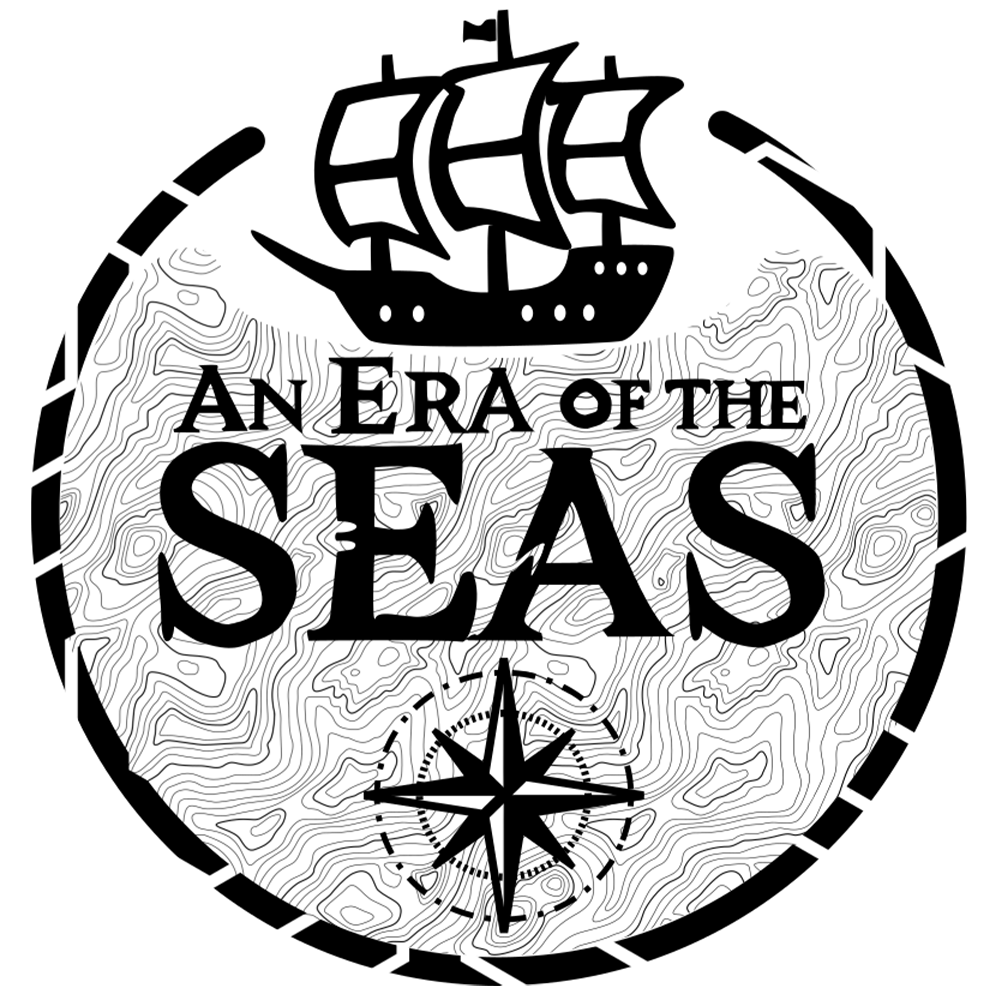
\includegraphics[width=3.5in]{AEotS Logo.png} \\
        \vspace{2cm}
        
\includegraphics[width=4in]{logo text.png}
    \end{minipage}
}
\date{}















\begin{document}

\maketitle

\vfill
\begin{center}
    \textbf{Lin Jérôme}\\
    \textbf{Ben Abdallah Achref}\\
    \textbf{Bruno Ethan}\\
    \textbf{Devin Joseph}\\
    \textbf{Class : A1}
\end{center}










\newpage
\thispagestyle{empty}
\addtocounter{page}{-1}
\null
\subsection*{Summary}
\tableofcontents










\newpage
\section{Introduction}\hfill

Welcome to \textit{An Era of the Seas}, an open-world adventure and exploration game where every island holds its mysteries, dangers… and opportunities. In this vast and living world, you play as the son of a debt-ridden merchant, determined to restore your family’s honor and fortune.\\

Your mission: explore the 8 islands of the archipelago, each with its own resources, inhabitants, challenges, and secrets. Whether through trading, treasure hunting, or battling enemies, every means is fair game to repay the family debt… and perhaps, along the way, forge your own legend.\\

Sail between islands, build your network, upgrade your ship, make tough decisions… The world of \textit{An Era of the Seas} is open, but unforgiving. The path you choose is yours alone.\\

\noindent Get ready to set sail. The adventure begins now.

\paragraph{About the Developers}\hfill

Dream Chasers is an independent studio driven by one passion: turning dreams into interactive worlds. For them, a video game is more than entertainment — it's an adventure, a story to live.\\

With \textit{An Era of the Seas}, their ambition is clear: to deliver an immersive experience blending exploration, realistic navigation, and strategic progression. This project reflects their commitment to pushing the boundaries of narrative gaming and crafting rich, captivating universes for players seeking escape.\\

\noindent Learn More about Dream Chasers and \textit{An Era of the Seas} at: \url{https://dream-chasers.odoo.com} 








\newpage
\section{Installation}\hfill
\paragraph{On Windows}\hfill
\begin{itemize}
    \item Download the installer (AnEraOfTheSeasSetup.exe)\\Source: \href{https://download1509.mediafire.com/8snf8hve0msgwdhdZEtEx8ZWzSdcMdMUCYDG2bgIvlOG-x9er_HSzQnK4Hep_nI6bvlHJN7dz2Sd6p5nzuyzCa4MUgP4R1LJcemgU61_V5KFJPmyTtjY-clWWBvB5S60wMG3_JgLnaoPeaz8tUJGs_yfov4AGlbom80quzQE0A_qinY/2ni5q6ldp0itobt/AnEraOfTheSeasSetup.exe}{https://www.mediafire.com/file/2ni5q6ldp0itobt/AnEraOfTheSeasSetup.exe/file}
    \item Run the installer (AnEraOfTheSeasSetup.exe) and follow the instructions
    \item Follow the instructions of the installer:
    \begin{itemize}
        \item Choose your preferred language
        \item Accept the terms and conditions
        \item Select the installation directory (default: \texttt{C:\textbackslash{}Program Files\textbackslash{}AnEraOfTheSeas})
        \item Choose whether to create a desktop shortcut or not by checking/unchecking the option
        \item Click Install
    \end{itemize}
    \item After installation:
    \begin{itemize}
        \item Optionally check "Launch An Era Of The Seas”
        \item Click Finish to close the installer
    \end{itemize}
\end{itemize}
You can launch the game in two ways:
\begin{itemize}
    \item From the desktop (if shortcut was created):\\Double-click the An Era Of the Seas icon.
    \item From the Start Menu:\\Go to Start $>$ An Era Of The Seas $>$ Open
\end{itemize}

\paragraph{On Linux}\hfill
\begin{itemize}
    \item \noindent Download the tar file (AnEraOfTheSeas.tar)\\Source: \href{https://download1474.mediafire.com/kfchuimtbalgux0CYxqvN47FxhO4syOjfBRZCmL-Id1E4w34gKKnELwd6J1gbhERWZ9EMc2zwXZgknoaO_KEtYnrX5A26h-LW-4u3VTocIizDK-iisEFy-cBh0hfv4zEzxYCq2eN-PsIGWjaJUOJDSgKFDXQ2XM7jTIqAyW_vFbYpz0/l0yk9sok3m1cj5l/AnEraOfTheSeas.tar}{https://www.mediafire.com/file/l0yk9sok3m1cj5l/AnEraOfTheSeas.tar/file}
    \begin{verbatim}
    tar -xvzf AnEraOfTheSeas.tar.gz
    cd AnEraOfTheSeas
    \end{verbatim}
    \item \noindent Make the main executable runnable:
    \begin{verbatim}
    chmod +x AnEraOfTheSeas.x86_64
    ./AnEraOfTheSeas.x86_64
    \end{verbatim}
\end{itemize}





\section{Uninstallation}
\paragraph{On Windows}\hfill

\noindent Open Control Panel $>$ Programs $>$ Uninstall a program\\
Select AnEraOfTheSeas and click Uninstall\\
Or:\\
Use the Uninstall AnEraOfTheSeas shortcut from the Start Menu

\paragraph{On Linux}
\begin{verbatim}
rm -rf ~/AnEraOfTheSeas/
rm -rf ~/.config/unity3d/DreamChasers/AnEraOfTheSeas/
\end{verbatim}










\newpage
\section{Commands}
\begin{table}[h]
    \begin{tabular}{|l|l|}
        \hline
        \textbf{Key} & \textbf{Action}\\
        \hline
        W / A / S / D & Move\\
        \hline
        Space Bar & jump\\
        \hline
        Mouse movement & Move camera\\
        \hline
        Left Click & Attack\\
        \hline
        E & Interact\\
        \hline
        B & Inventory\\
        \hline
        M & Map\\
        \hline
        H & Place/Remove Boat\\
        \hline
        R & Eat\\
        \hline
        X & Exit Boat\\
        \hline
        ESC & Return/Settings\\
        \hline
    \end{tabular}
\end{table}





\section{User Interface}\hfill
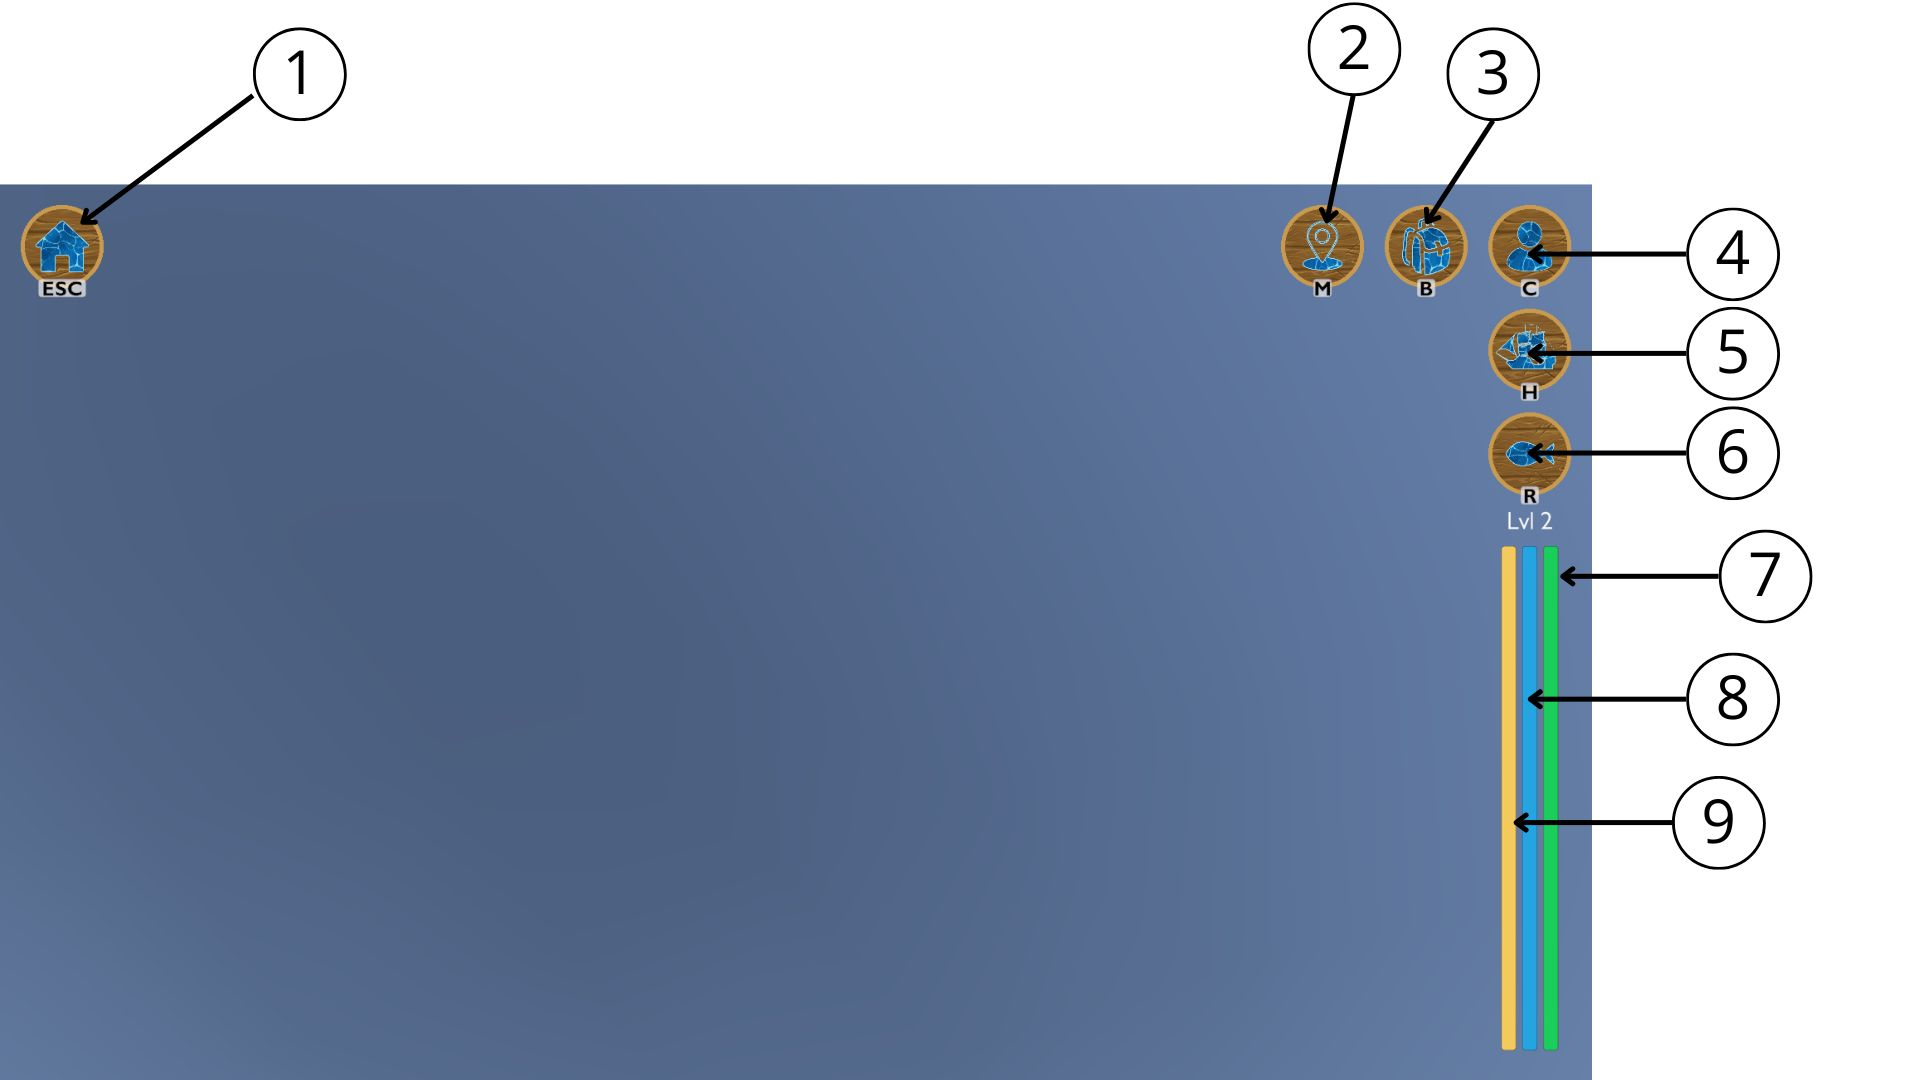
\includegraphics[width=6in]{UI.jpg}\\
1: Settings\\
2: Map\\
3: Inventory\\
4: Equipment\\
5: Place/Remove Boat\\
6: Eat\\
7: Health Bar\\
8: Defense Bar\\
9: Hunger Bar










\newpage
\section{Game Mechanics}\hfill
\subsection{Quests \& Story Progression}
The player embarks on a journey as the son of a vanished merchant burdened by debt. Set in the mysterious world of the Shattered Seas, the player’s goal is to gain power and wealth. The main storyline unfolds through a Story Quest, where players interact with NPCs and explore diverse islands to uncover the fate of their family and the secrets of the seas.

\subsection{Combat System}
Combat in Shattered Seas is divided into two main types:
\begin{itemize}
    \item \textbf{Land Combat}: Engage enemies on foot using your sword in real-time battles. Defeating enemies may yield valuable loots and resources.
    \item \textbf{Naval Combat}: Battle maritime foes aboard your ship. Maneuver your vessel and defeat the enemies to claim rewards.
\end{itemize}

\subsection{Exploration}
Exploration plays a crucial role in your journey to grow stronger and wealthier. Travel from island to island by boat and face new enemies.

\subsection{Upgrades}
Players can enhance their strength by upgrading:
\begin{itemize}
    \item Weapons
    \item Sigils
    \item Boats
    \item Crew Members
\end{itemize}
Upgrades improve stats such as damage, health, and defense.
Upgrade materials include:
\begin{itemize}
    \item Coins and Pure Water Drop for general upgrades
    \item Wood and Steel for boat enhancements
\end{itemize}
Advanced gear and upgrade items can be purchased from shops located in the central towns of each island.

\subsection{Hunger system}
Managing your character’s Hunger bar is essential for survival:
\begin{itemize}
    \item When full, it regenerates health over time.
    \item When empty, the player gradually loses health.
\end{itemize}
Players can fish at designated spots and consume the catch to restore hunger and stay in fighting shape.

\subsection{Shop}
Each island town features a variety of shops where players can buy or sell equipment and manage their resources:
\begin{itemize}
    \item \textbf{Armorer} - Sells weapons
    \item \textbf{Mage} - Offers magical sigils
    \item \textbf{Boat Dealer} - Provides ships and naval upgrades
    \item \textbf{Material Seller} - Sells crafting materials (Pure Water Drop, Steel, Wood)
    \item \textbf{Crew Agent} - Recruits crew members to join your ship, each with unique skills and roles
    \item \textbf{Purchaser} - Buys any items and offers money or Pure Water Drop depending on the trade
\end{itemize}
Managing your economy effectively is key to progression and survival.

\subsection{Multiplayer}
Players can enjoy local multiplayer through two competitive mini-games:
\begin{itemize}
    \item \textbf{Treasure Hunt} - Compete to find the hidden treasure chest first.
    \item \textbf{Boat Race} - Navigate through a challenging course; the first to capture the final flag wins.
\end{itemize}
These modes offer fun, fast-paced gameplay for friends on the same system.










\newpage
\section{License}
End-User License Agreement (EULA)\\
\newline
\noindent This game is licensed, not sold. By installing or using the software, you agree to the following terms:\\
1. You may use this software for personal entertainment.\\
2. You may not redistribute, modify, or decompile this software.\\
3. All content, including code, art, and audio, is owned by Dream Chasers.\\
4. This software is provided "as is", without warranty of any kind.\\
\newline
\noindent © 2025 Dream Chasers. All rights reserved.















\end{document}